\section{Experiments and results}
\label{sec:results}

The Virtual KITTI 3D Dataset is split into 6 different point clouds. For our experiments, we used 5 for training the neural network and 1 for testing it. Below there are some of our results. In pictures \ref{res_true} and \ref{res1_pred}, we can see the result is not visually pleasing but overall, the algorithm seems to distinguish easily the trees from the rest. We can also see that a pole in the left side is quite recognizable. However, in picture \ref{res2_pred}, we begin to see better classification. It gives us good hope on the algorithm, since picture \ref{res2_pred} was computed on more samples (but more unbalanced). Then, we might think that with more balanced data, we could achieve expected results.\\

We explain the quality of our results by the strong imbalance of our dataset. We logged information about our training dataset in \verb|.info| files and we saw that the tree classs is the most predominant one. It is then difficult to have training samples balanced over all the labels. The authors took 50000 balanced training samples, and we have barely 20000 samples, which are not even well balanced. Another issue is the required computing power: we lack a beautiful RTX 2080 Ti and some RAM. But we managed to use Google Colab to train some models and obtain some results.

\begin{figure}[H]
    \centering
	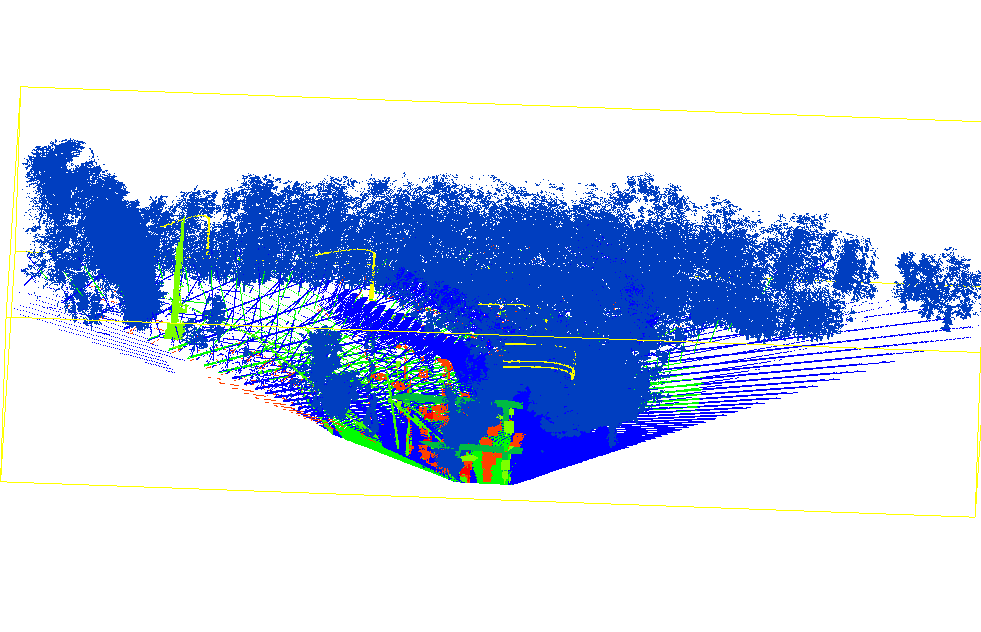
\includegraphics[scale=0.27]{sources/res_true.png}
	\caption{Experiment 1: true labels}
	\label{res_true}
\end{figure}

\begin{figure}[H]
    \centering
	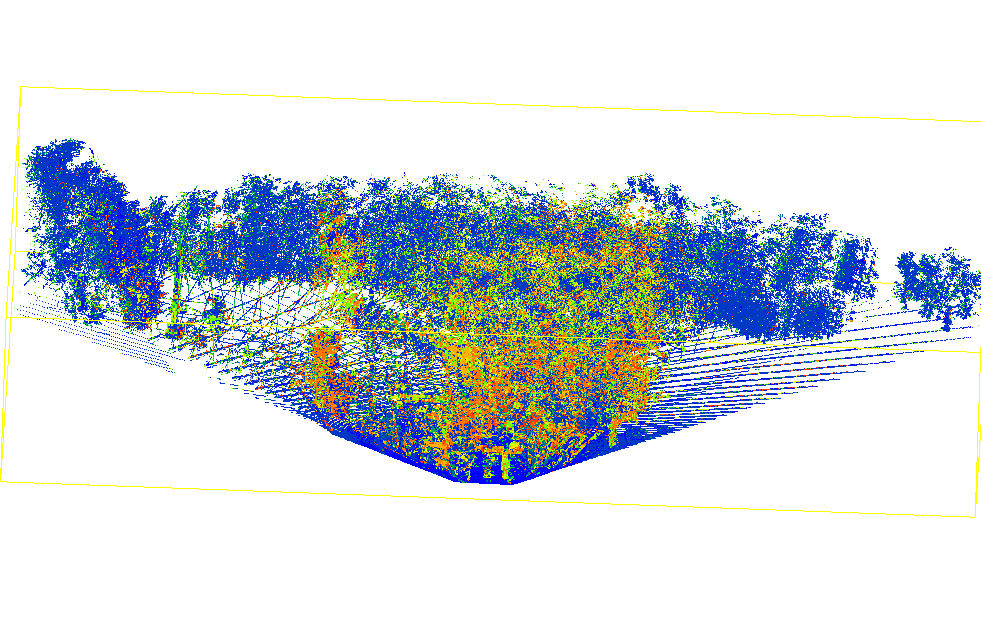
\includegraphics[scale=0.27]{sources/res1_pred.png}
	\caption{Experiment 1: predicted labels}
	\label{res1_pred}
\end{figure}

\begin{figure}[H]
    \centering
	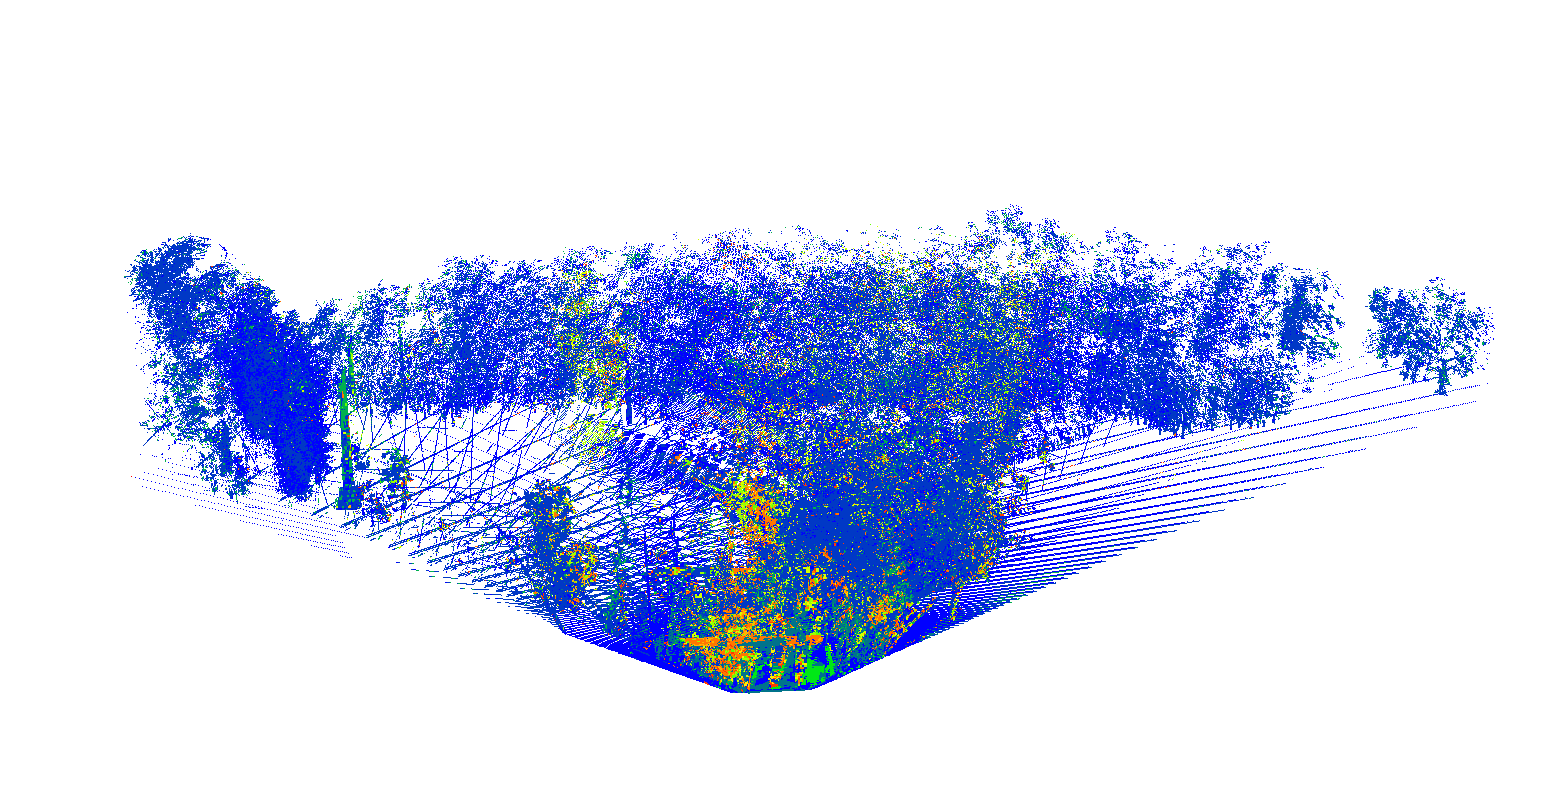
\includegraphics[scale=0.27]{sources/res2_pred.png}
	\caption{Experiment 1: predicted labels}
	\label{res2_pred}
\end{figure}
